\documentclass[12pt]{letter}
\usepackage{amsmath,amsfonts,amsthm,amstext,amssymb,graphicx, multicol,fancyhdr,lastpage,fullpage,framed,fancybox,enumerate,tikz,color,mathrsfs, polynom}
\usepackage[margin=0.6in,headsep=3pt, headheight=15pt]{geometry}

% ----------------------------------------------------------
% Custom Definitions, Commands, Environments, etc.

% Sets of numbers
\def\R{\mathbb{R}} % The reals
\def\N{\mathbb{N}} % The naturals
\def\Z{\mathbb{Z}} % The integers
\def\Q{\mathbb{Q}} % The rationals

% Blank space
\newcommand{\blank}[1]{\underline{\hspace{#1}}} % Blank space

% Change font colors
\newcommand{\cyan}[1]{{\color{cyan}{#1}}} % Changes font to cyan
\newcommand{\red}[1]{{\color{red}{#1}}} % Changes font to red
\newcommand{\magenta}[1]{{\color{magenta}{#1}}} % Changes font to magenta
\newcommand{\orange}[1]{{\color{orange}{#1}}} % Changes font to orange
\newcommand{\yellow}[1]{{\color{yellow}{#1}}} % Changes font to yellow
\newcommand{\violet}[1]{{\color{violet}{#1}}} % Changes font to violet
\newcommand{\green}[1]{{\color{green}{#1}}} % Changes font to green
\newcommand{\blue}[1]{{\color{blue}{#1}}} % Changes font to blue
\newcommand{\white}[1]{{\color{white}{#1}}} % Changes font to white

% Fitted inclusion symbols
\newcommand{\fp}[1]{\left({#1}\right)} % Fitted parentheses around content
\newcommand{\fb}[1]{\left[{#1}\right]} % Fitted brackets
\newcommand{\set}[1]{\left\{{#1}\right\}} % Fitted braces (useful for sets)
\newcommand{\av}[1]{\left|{#1}\right|} % Fitted absolute value bars

% Augmented Matrix Environment
\newenvironment{amatrix}[1]{%
	\left[\begin{array}{@{}*{#1}{c}|c@{}}
	}{%
	\end{array}\right]
}

% Miscellaneous
\def\then{\Rightarrow}
\def\to{\rightarrow}
\def\d{^{\circ}}
\newcommand{\?}{\stackrel{?}{=}}



% Coordinate Plane (Four-Quadrant)
\def\coordplane {
	\begin{tikzpicture}		\draw[step=0.25cm,black,very thin,opacity=0.25] (-2.5cm, -2.5cm) grid (2.5cm, 2.5cm);
	\draw[<->,thick,black] (-2.5cm, 0) -- (2.5cm, 0) node[anchor=north west,pos=0.94,font=\scriptsize]{$x$};
	\draw[<->,thick,black] (0,-2.5cm) -- (0, 2.5cm) node[anchor=south east,font=\scriptsize,pos=0.94]{$y$};
	\end{tikzpicture}
}

% Coordinate Plane (One-Quadrant)
\def\onequad {
	\begin{tikzpicture}
	\draw[step=0.25cm, black, very thin, opacity=0.25] (0,0) grid (7.5cm,5cm);
	\draw[->, thick, black] (0,0) -- (7.5cm, 0) node[anchor=north west,font=\scriptsize,pos=0.94]{$x$};
	\draw[->, black, thick] (0,0) -- (0,5cm) node[anchor=south east,font=\scriptsize,pos=0.94]{$y$};
	\end{tikzpicture}
}

% Counters
\newcounter{exercise}

% Exercise environment (auto-numbered)
\newenvironment{exercise}[1][]{\begin{framed}\refstepcounter{exercise}\textbf{Exercise~\theexercise:} #1}{\end{framed}}

% Book exercise environment
\newenvironment{bex}[2][] {
	\begin{framed}
		\textbf{Book Exercise {#2}}#1
	\end{framed}
}
% ----------------------------------------------------------

% ----------------------------------------------------------
% Header and Footer Information
% \pagestyle{fancy}
% \fancyhf{}
% \renewcommand{\headrulewidth}{0pt}
% \rhead{Name: \blank{2in}}
% \lhead{@}
% \rfoot{Page \thepage \, of \,\pageref{LastPage}}
% ----------------------------------------------------------
\author{Jacob Ayers}

\begin{document}
	\textbf{Assignment 10 Key \\ MAT 130}
	
	\begin{bex}{5.4.22}
		{
			
		}
	\end{bex} \vspace{-32pt}
	
	% My answer here
	\begin{flalign*}
	4e^x &= 91 & \\
	e^x &= \dfrac{91}{4} & \\
	x &= \ln \dfrac{91}{4} & \\
	x &\approx 3.125
	\end{flalign*}
	
	\vfill % \newpage
	
	\begin{bex}{5.4.26}
		{
			
		}
	\end{bex} \vspace{-32pt}
	
	% My answer here
	\begin{flalign*}
	4^{-3t} &= 0.10 & \\
	-3t &= \log_4 0.10 & \\
	-3t &= \dfrac{\log_0.10}{\log 4} & \\
	-3t &\approx -1.660964047 & \\
	t &\approx 0.554
	\end{flalign*}
	
	\vfill % \newpage
	
	\begin{bex}{5.4.30}
		{
			
		}
	\end{bex} \vspace{-32pt}
	
	% My answer here
	\begin{flalign*}
	8\fp{3^{6 - x}} &= 40 & \\
	3^{6 - x} &= 5 & \\
	6 - x &= \log_3 5 & \\
	6 - x &= \dfrac{\log 5}{\log 3} & \\
	6 - x &\approx 1.464973521 & \\
	-x &\approx -4.535026479 & \\
	x &\approx 4.535
	\end{flalign*}
	
	\vfill % \newpage
	
	\begin{bex}{5.4.34}
		{
			
		}
	\end{bex} \vspace{-32pt}
	
	% My answer here
	\begin{flalign*}
	-14 + 3e^x &= 11 & \\
	3e^x &= 25 & \\
	e^x &= \dfrac{25}{3} & \\
	x &= \ln\dfrac{25}{3} & \\
	x &\approx 2.120
	\end{flalign*}
	
	\vfill \newpage
	
	\begin{bex}{5.4.38}
		{
			
		}
	\end{bex} \vspace{-32pt}
	
	% My answer here
	\begin{flalign*}
	e^{x + 1} &= 2^{x + 2} & \\
	x + 1 &= \ln \fp{2^{x + 2}} & \\
	x + 1 &= \fp{x+2}\ln 2 & \\
	x + 1 &= x\ln 2 + 2\ln 2 & \\
	x - x\ln 2 &= 2\ln 2 - 1
	x\fp{1 - \ln 2} &= 2\ln 2 - 1 & \\
	x &= \dfrac{2\ln 2 - 1}{1 - \ln 2} & \\
	x &\approx 1.259
	\end{flalign*}
	
	\vfill % \newpage
	
	\begin{bex}{5.4.42}
		{
			
		}
	\end{bex} \vspace{-8pt}
	
	% My answer here
	Let $u = e^x$. \begin{flalign*}
	e^{2x} - 5e^x + 6 &= 0 & \\
	u^2 - 5u + 6 &= 0 & \\
	(u - 3)(u - 2) &= 0 & \\
	u &= \set{2, 3}
	\end{flalign*}
	$e^x = 2 \then x = \ln 2 \approx 0.693$ \\
	$e^x = 3 \then x = \ln 3 \approx 1.099$ \\
	$x \approx \set{0.693, 1.099}$
	
	\vfill % \newpage
	
	\begin{bex}{5.4.48}
		{
			
		}
	\end{bex} \vspace{-32pt}
	
	% My answer here
	\begin{flalign*}
	\ln x - 7 &= 0 & \\
	\ln x &= 7 & \\
	e^7 &= x & \\
	x &\approx 1096.633
	\end{flalign*}
	
	\vfill % \newpage
	
	\begin{bex}{5.4.52}
		{
			
		}
	\end{bex} \vspace{-32pt}
	
	% My answer here
	\begin{flalign*}
	3 + 8\ln x &= 7 & \\
	8 \ln x &= 4 & \\
	\ln x &= \dfrac12 & \\
	e^{1/2} &= x & \\
	x &\approx 1.649
	\end{flalign*}
	
	\vfill \newpage
	
	\begin{bex}{5.4.56}
		{
			
		}
	\end{bex} \vspace{-32pt}
	
	% My answer here
	\begin{flalign*}
	\ln x + \ln (x + 1) &= 1 & \\
	\ln\fb{x\fp{x+1}} &= 1 & \\
	x\fp{x + 1} &= e^1 & \\
	x^2 + x &= e & \\
	x^2 + x - e &= 0 & \\
	x &= \dfrac{-1\pm\sqrt{1^2 - 4(1)(-e)}}{2(1)} & \\
	x &\approx \dfrac{-1\pm\sqrt{11.87312731}}{2} & \\
	x &\approx \dfrac{-1 + \sqrt{11.87312731}}{2} \approx 1.223 & \\
	x &\approx \dfrac{-1 - \sqrt{11.87312731}}{2} \approx -2.223
	\end{flalign*}
	However, the solution $-2.223$ does not work in the original equation because it is impossible to evaluate $\ln -2.223$. So there is only one solution: $x \approx 1.223$.
	
	\vfill % \newpage
	
	\begin{bex}{5.4.58}
		{
			
		}
	\end{bex} \vspace{-32pt}
	
	% My answer here
	\begin{flalign*}
	\ln (x + 1) - \ln (x - 2) &= \ln x & \\
	\ln \dfrac{x+1}{x - 2} &= \ln x & \\
	\dfrac{x+1}{x-2} &= x & \\
	x + 1 &= x\fp{x - 2} & \\
	x +1 &= x^2 - 2x & \\
	x^2 - 3x - 1 &= 0 & \\
	x &= \dfrac{3\pm\sqrt{(-3)^2 - 4(1)(-1)}}{2(1)} & \\
	x &= \dfrac{3\pm\sqrt{13}}{2} & \\
	x &= \dfrac{3 + \sqrt{13}}{2} \approx 3.303
	\end{flalign*}
	The other root will not make sense since $\dfrac{3 - \sqrt{13}}{2} < 0$. There is only one solution: $x \approx 3.303$
	
	\vfill \newpage
	
	\begin{bex}{5.4.60}
		{
			
		}
	\end{bex} \vspace{-32pt}
	
	% My answer here
	\begin{flalign*}
	\log_2 x + \log_2 (x + 2) &= \log_2 (x+6) & \\
	\log_2 \fb{x\fp{x + 2}} &= \log_2 (x+6) & \\
	x(x+2) &= x+6 & \\
	x^2 + 2x = x + 6 & \\
	x^2 + x - 6 &= 0 & \\
	(x + 3)(x - 2) &= 0 & \\
	x &= \set{-3, 2}
	\end{flalign*}
	But the solution $x = -3$ does not make sense; the only solution is $x = 2$.
	
	\vfill % \newpage
	
	\begin{bex}{5.4.72}
		{
			
		}
	\end{bex} \vspace{-8pt}
	
	% My answer here
	(a) \begin{flalign*}
	5000 &= 2500e^{0.0375t} & \\
	2 &= e^{0.0375t} & \\
	0.0375t &= \ln 2 & \\
	t &= \dfrac{\ln 2}{0.0375} & \\
	&\approx 18.484 \text{ yr}
	\end{flalign*}
	(b) \begin{flalign*}
	7500 &= 2500e^{0.0375t} & \\
	3 &= e^{0.0375t} & \\
	0.0375t &= \ln 3 & \\
	t &= \dfrac{\ln 3}{0.0375} & \\
	&\approx 29.296 \text{ yr}
	\end{flalign*}
	
	\vfill \newpage
	
	\begin{bex}{5.4.82}
		{
			
		}
	\end{bex} \vspace{-8pt}
	
	% My answer here
	(a) \begin{flalign*}
	169 &= 5000\fp{1 - \dfrac{4}{4 + e^{-0.002x}}} & \\
	0.0338 &= 1 - \dfrac{4}{4 + e^{-0.002x}} & \\
	-0.9662 &= -\dfrac{4}{4 + e^{-0.002x}} & \\
	-0.9662\fp{4 + e^{-0.002x}} &= -4 & \\
	-3.8648 - 0.9662e^{-0.002x} &= -4 & \\
	-0.9662e^{-0.002x} &= -0.1352 & \\
	e^{-0.002x} &= 0.1399296212 & \\
	-0.002x &= \ln 0.1399296212 & \\
	x &= \dfrac{\ln 0.1399296212}{-0.002} & \\
	&\approx 983.308 \text{ units}
	\end{flalign*}
	(b) \begin{flalign*}
	299 &= 5000\fp{1 - \dfrac{4}{4 + e^{-0.002x}}} & \\
	0.0598 &= 1 - \dfrac{4}{4 + e^{-0.002x}} & \\
	-0.9402 &= -\dfrac{4}{4 + e^{-0.002x}} & \\
	-0.9402\fp{4 + e^{-0.002x}} &= -4 & \\
	-3.7608 - 0.9402e^{-0.002x} &= -4 & \\
	-0.9402e^{-0.002x} &= -0.2392 & \\
	e^{-0.002x} &= 0.2544139545 & \\
	-0.002x &= \ln 0.2544139545 & \\
	x &= \dfrac{\ln 0.2544139545}{-0.002} & \\
	&\approx 684.396 \text{ units}
	\end{flalign*}
	
	\vfill \newpage
	
	\begin{bex}{5.4.86}
		{
			
		}
	\end{bex} \vspace{-32pt}
	
	% My answer here
	\begin{flalign*}
	965 &= 81\ln t + 807 & \\
	81\ln t &= 158 & \\
	\ln t &= \dfrac{158}{81} & \\
	e^{158/81} &= t & \\
	t &\approx 7.033
	\end{flalign*}
	The population of Montana exceeded 965 thousand in 2007.
	
	\vfill % \newpage
	
	\begin{bex}{5.5.30}
		{
			
		}
	\end{bex} \vspace{-8pt}
	
	% My answer here
	\textbf{\underline{Bulgaria}}
	\begin{flalign*}
	7.2 &= ae^{15b} \then a = 7.2e^{-15b} & \\
	6.7 &= ae^{25b} & \\
	6.7 &= 7.2e^{-15b}e^{25b} & \\
	\dfrac{67}{72} &= e^{10b} & \\
	10b &= \ln \dfrac{67}{72} & \\
	b &= \dfrac{\ln\frac{67}{72}}{10} \approx -0.00720 & \\
	a &= 7.2e^{-15(-0.00720)} \approx 8.021
	\end{flalign*}
	Model for Bulgaria: $y = 8.021e^{-0.00720t}$ \\
	Population in 2035: $y = 8.021e^{-0.00720(35)} \approx 6.2$ million
	
	\textbf{\underline{Canada}} \begin{flalign*}
	35.1 &= ae^{15b} \then a = 35.1e^{-15b} & \\
	37.6 &= ae^{25b} & \\
	37.6 &= 35.1e^{10b} & \\
	\dfrac{376}{351} &= e^{10b} & \\
	10b &= \ln\dfrac{376}{51} & \\
	b &= \dfrac{\ln \frac{376}{351}}{10} \approx 0.00688 & \\
	a &= 35.1e^{-15(0.00688)} \approx 31.658
	\end{flalign*}
	Model for Canada: $y = 31.658e^{0.00688t}$ \\
	Population in 2035: $y = 31.658e^{0.00688(35)} \approx 40.3$ million
	
	\vfill \newpage
	
	\textbf{\underline{China}} \begin{flalign*}
	1367.5 &= ae^{15b} \then a = 1367.5e^{-15b} & \\
	1407 &= ae^{25b} & \\
	1407 &= 1367.5e^{10b} & \\
	\dfrac{14070}{13675} &= e^{10b} & \\
	b &= \dfrac{\ln\frac{14070}{13675}}{10} \approx 0.00285 & \\
	a &= 1367.5e^{-15(0.00285)} \approx 1310.319
	\end{flalign*}
	Model for China: $y = 1310.319e^{0.00285t}$ \\
	Population in 2035: $y = 1310.319e^{0.00285(35)} \approx 1447.7$ million
	
	\textbf{\underline{United Kingdom}} \begin{flalign*}
	64.1 &= ae^{15b} \then a = 64.1e^{-15b} & \\
	67.2 &= ae^{25b} & \\
	67.2 &= 64.1e^{10b} & \\
	\dfrac{672}{641} &= e^{10b} & \\
	b &= \dfrac{\ln\frac{672}{641}}{10} \approx 0.00472 & \\
	a &= 64.1e^{-15(0.00472)} \approx 59.716
	\end{flalign*}
	Model for UK: $y = 59.716e^{0.00472t}$ \\
	Population in 2035: $y = 59.716e^{0.00472(35)} \approx 70.4$ million
	
	\textbf{\underline{United States}}
	\begin{flalign*}
	321.4 &= ae^{15b} \then a = 321.4e^{-15b} & \\
	347.3 &= ae^{25b} & \\
	347.3 &= 321.4e^{10b} & \\
	\dfrac{3743}{3214} &= e^{10b} & \\
	b &= \dfrac{\ln\frac{3743}{3214}}{10} \approx 0.00775 & \\
	a &= 321.4e^{-15(0.00775)} \approx 286.126
	\end{flalign*}
	Model for US: $y = 286.126e^{0.00775t}$ \\
	Population in 2035: $y = 286.126e^{0.00775t} \approx 375.2$ million
	
	(b) The constant $b$ gives the growth rate. When $b > 0$, the population is growing and when $b < 0$ the population is decreasing. The larger the magnitude of $b$, the more quickly the population is changing.
	\vfill \newpage
	
	\begin{bex}{5.5.32}
		{
			
		}
	\end{bex} \vspace{-8pt}
	
	% My answer here
	(a) \begin{flalign*}
	163.075 &= 150.9e^{5k} & \\
	\dfrac{163075}{150900} &= e^{5k} & \\
	5k &= \ln \dfrac{163075}{150900} & \\
	k &= \dfrac{\ln\frac{163075}{150900}}{5} \approx 0.0155
	\end{flalign*}
	Since $k > 0$, the population of Tallahassee is increasing (by about 1.55\% each year).
	
	(b) Using a graphing calculator:
	
	\begin{tabular}{c|cc}
		Year & 2020 & 2025 \\ \hline
		Population (thousands) & 205.817 & 222.423
	\end{tabular}

	This seems reasonable. It is likely that the population of the city will continue to increase over time.
	
	(c) \begin{flalign*}
	200 &= 150.9e^{0.0155t} & \\
	\dfrac{2000}{1509} &= e^{0.0155t} & \\
	0.0155t &= \ln \dfrac{2000}{1509} & \\
	t &= \dfrac{\ln \frac{2000}{1509}}{0.0155} \approx 18.174
	\end{flalign*}
	The population will reach 200,000 in 2018.
	
	\vfill % \newpage
	
	\begin{bex}{5.5.34}
		{
			
		}
	\end{bex} \vspace{-8pt}
	
	% My answer here
	First, we need to find a model. Once we've found a model, we plan substitute $t = 6$ to find the number of bacteria after 6 hours. Since the population is growing according to the law of exponential growth, our model will be of the form $y = ae^{bt}$, where $a$ is the initial population and $b$ is the growth factor. We know that $a = 250$ and that when $t = 10$, $y = 500$.
	\begin{flalign*}
	500 &= 250e^{10b} & \\
	2 &= e^{10b} & \\
	10b &= \ln 2 & \\
	b &= \dfrac{\ln 2}{10} \approx 0.0693
	\end{flalign*}
	Our model is $y = 250e^{0.0693t}$. So when $t = 6$, the population was \\
	$y = 250e^{6(0.0693)} \approx 378.929$ bacteria.
	
	\vfill \newpage
	
	\begin{bex}{5.5.36}
		{
			
		}
	\end{bex} \vspace{-8pt}
	
	% My answer here
	(a) We have that $N = 19$ when $t = 20$. \begin{flalign*}
	19 &= 30\fp{1 - e^{20k}} & \\
	\dfrac{19}{30} &= 1 - e^{20k} & \\
	-\dfrac{11}{30} &= -e^{20k} & \\
	\dfrac{11}{30} &= e^{20k} & \\
	\ln \dfrac{11}{30} &= 20k & \\
	k &= \dfrac{\ln\frac{11}{30}}{20} \approx -0.0502
	\end{flalign*}
	The learning curve for this employee is $N = 30\fp{1 - e^{-0.0502t}}$.
	
	(b) We want to know when $N = 25$. \begin{flalign*}
	25 &= 30\fp{1 - e^{-0.0502t}} & \\
	\dfrac{5}{6} &= 1 - e^{-0.0502t} & \\
	\dfrac16 &= e^{-0.0502t} & \\
	-0.0502t &= \ln\dfrac16 & \\
	t &= \dfrac{\ln\frac16}{-0.0502} \approx 35.717 
	\end{flalign*}
	After about 36 days, the employee will be producing 25 units per day.
	
	\vfill % \newpage
	
	\begin{bex}{5.5.38}
		{
			
		}
	\end{bex} \vspace{-8pt}
	
	% My answer here
	The carbon dating model is $R = \dfrac{1}{10^{12}}e^{-x/8223}$. \begin{flalign*}
	\dfrac{1}{13^{11}} &= \dfrac{1}{10^{12}}e^{-x/8223} & \\
	\dfrac{10^{12}}{13^{11}} &= e^{-x/8223} & \\
	0.5579857714 &= e^{-x/8223} & \\
	-\dfrac{x}{8223} &= \ln 0.5579857714 & \\
	x &\approx 4797.478 
	\end{flalign*}
	The piece of paper is about 4797 years old.
	
	\vfill \newpage
	
	\begin{bex}{5.5.40}
		{
			
		}
	\end{bex} \vspace{-8pt}
	
	% My answer here
	(a) 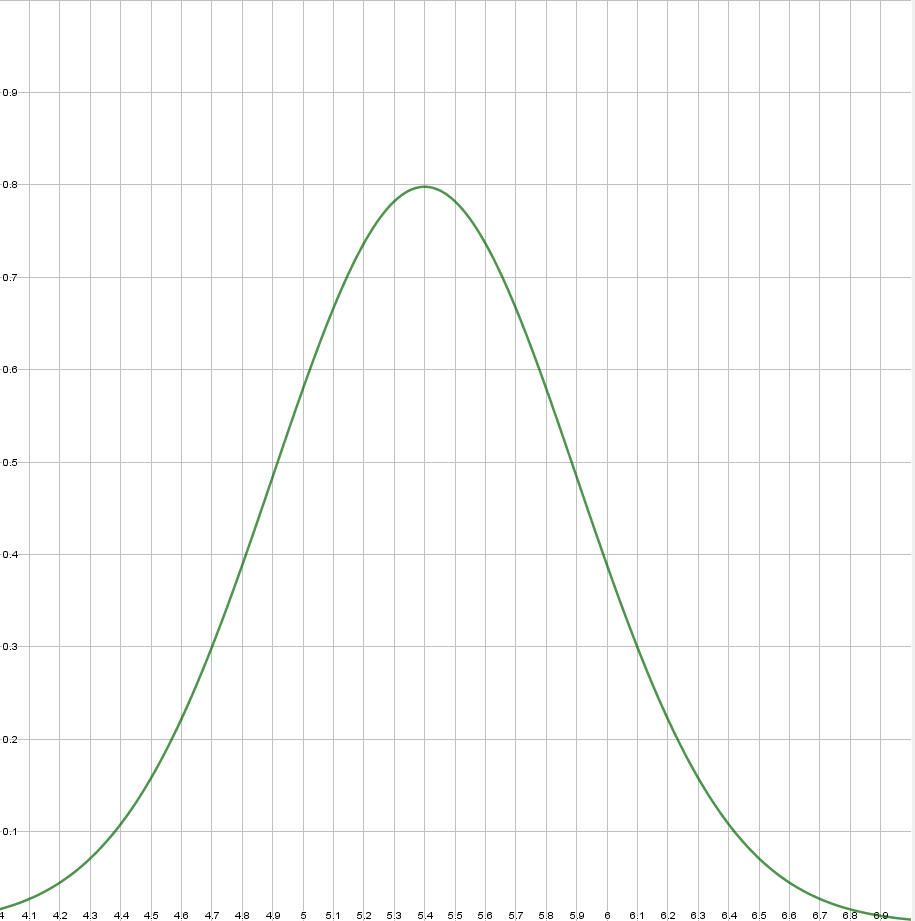
\includegraphics[width=3in]{5540a.png}
	
	(b) The average number of hours per week a student uses the tutoring center is about 5.4.
	
	\vfill % \newpage
	
	\begin{bex}{5.5.42}
		{
			
		}
	\end{bex} \vspace{-8pt}
	
	% My answer here
	(a) Using a graphing calculator:
	
	\begin{tabular}{c|cccc}
		Year & 2000 & 2005 & 2010 & 2015 \\ \hline
		Population (thousands) & 2430.3 & 2378.5 & 2315.2 & 2238.6
	\end{tabular}

	(b) 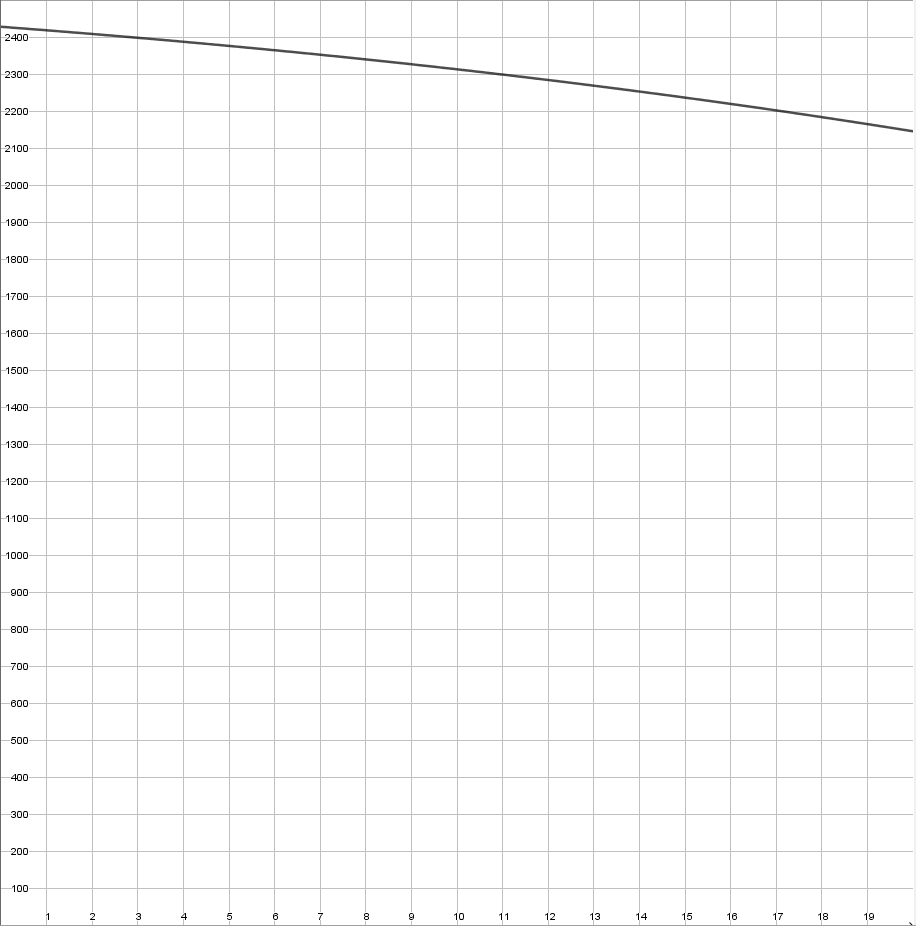
\includegraphics[width=3in]{5542b.png}

	(c) Note that 2.2 million is 2200 thousand; $P$ appears to be at 2200 when $t = 17$ so the population reached 2.2 million in 2017.
	
	\vfill \newpage
	
	(d) \begin{flalign*}
	2200 &= \dfrac{2632}{1 + 0.083e^{0.050t}} & \\
	2200\fp{1 + 0.083e^{0.050t}} &= 2632 & \\
	1 + 0.083e^{0.050t} &= \dfrac{2632}{2200} & \\
	0.083e^{0.050t} &= 0.196\overline{36} \\
	e^{0.050t} &= 2.365826944 & \\
	0.050t &= \ln 2.363826944 & \\
	t &= \dfrac{\ln 2.363826944}{0.050} \approx 17.223
	\end{flalign*}
	
	\vfill % \newpage
	
	\begin{bex}{5.5.44}
		{
			
		}
	\end{bex} \vspace{-8pt}
	
	% My answer here
	(a) It appears that about 40,000 units were sold in 2020.
	
	(b) \begin{flalign*}
	300000 &= \dfrac{500000}{1 + 0.1e^{4k}} & \\
	300000\fp{1 + 0.1e^{4k}} &= 500000 & \\
	1 + 0.1e^{4k} &= 1.\overline{6} & \\
	0.1e^{4k} &= 0.\overline{6} & \\
	e^{4k} &= 6.\overline{6} & \\
	4k &= \ln 6.\overline{6} & \\
	k &= \dfrac{\ln 6.\overline{6}}{4} \approx 0.474
	\end{flalign*}
	The model is $S = \dfrac{500000}{1 + e^{0.474t}}$.
	
	(c) $S = \dfrac{500000}{1 + 0.1e^{10(0.474)}} \approx 40078.534$ units, which is close to the estimate we made in part (a).
	
	\vfill \newpage
	
	\begin{bex}{5.5.58}
		{
			
		}
	\end{bex} \vspace{-8pt}
	
	% My answer here
	In our model, we have that $P = 120000$, $r = 0.075$, and $M = 839.06$. 
	
	(a) $u$ is represented by the red curve and $v$ is represented by the blue curve.
	
	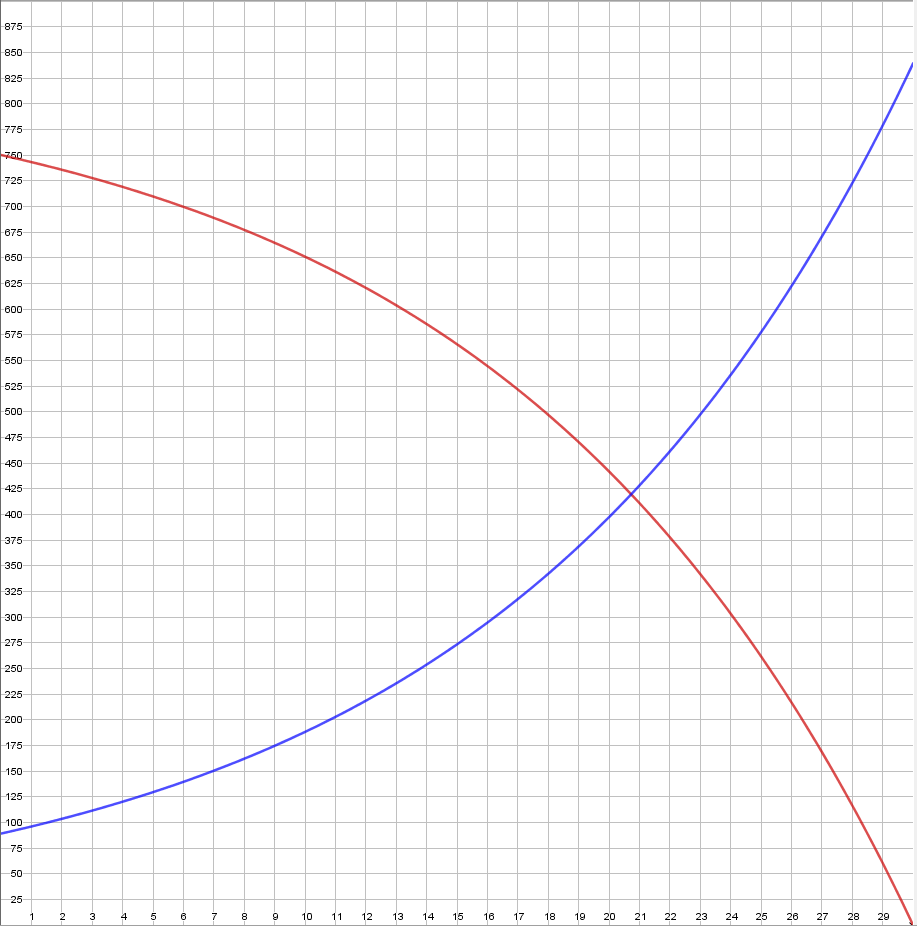
\includegraphics[width=3in]{5558a.png}
	
	(b) Early in the life of the loan, the red line (interest) is well above the blue line (principal). At about 21 years, the amount of interest and the amount of principal of the payment are the same. So for most of the loan, you're paying more interest than principal.
	
	\vfill \newpage
	
	(c) Changing the monthly payment changes the graph:
	
	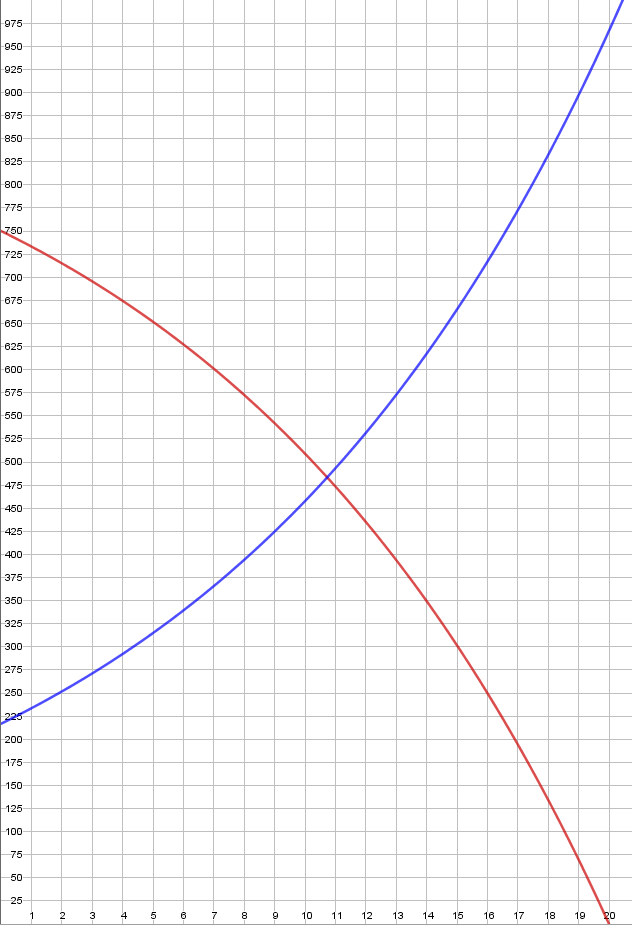
\includegraphics[width=3in]{5558c.png}
	
	Notice that the interest and principal are now the same just 11 years into the mortgage. If you take a shorter mortgage, then you'll pay less in interest, but you'll have a higher monthly payment. \\ \hrule
	
	Aside: The phenomenon you saw in this problem is called \textit{amortization} - no matter what type of home loan you get, your payment breakdowns will look similar to this one. Most first-time homeowners get a 30-year fixed mortgage because they haven't built up a ton of assets. There's nothing wrong with a 30-year mortgage, but you generally get a better interest rate, and pay less for the loan over its life, if you can afford to make the higher payments on a loan with a shorter term. Here's the cost breakdown for this case:
	
	30 years: $839.06\times 360 = 302061.60$ \\
	20 years: $966.71 \times 240 = 232010.40$
	
	You save over \$70,000 by paying the extra \$127.65 per month, but not everyone is able to afford to pay an extra \$100+ per month. Someday when you are getting ready to buy a house, it will be very helpful for you to have a budget in place so that you know how much home you can afford! The mortgage payment isn't the whole picture, either - you also have to pay homeowners insurance and property taxes. I personally bought a house recently. My mortgage payment is only \$428 per month, but with property taxes and homeowner's insurance, I pay about \$740 per month.
	
	
\end{document}